%!TeX spellcheck = fr_FR
\documentclass[letterpaper, 12pt]{article}
\usepackage[top = 1.6cm, left = 2cm, right = 2cm ]{geometry}
\usepackage[pdftex]{graphicx}
\usepackage{soulutf8}
\usepackage{amsmath}
\usepackage{tikz}
\usepackage[utf8]{inputenc}
\usepackage{longtable}
\usepackage[T1]{fontenc}
\usepackage{epigraph}
\usepackage{fancyhdr}
\usepackage{float}
\usepackage{subfig}
\usepackage{xcolor}
\usepackage{eurosym}
\usepackage{calc}
\usepackage{multirow} 
%
%
%%%%% Custom commands
%
%
\def\changemargin#1#2{\list{}{\rightmargin#2\leftmargin#1}\item[]}
\let\endchangemargin=\endlist 
%
\newcommand{\newlinealinea}{
~\\ \hspace*{0.5cm}}
%
\newcommand{\alinea}{
\hspace*{0.5cm}}
%
\newcommand{\alinealong}{
\hspace*{1.1cm}}
%
\newcommand{\alignparagraph}{
\hspace*{0.6cm}}
%
\newcommand{\red}[1]{
	\textcolor{red}{#1}}
%
\newcommand{\green}[1]{
	\textcolor{green}{#1}}
%
\newcommand{\point}{$\bullet\ $}
%
\makeatletter
	\newcommand*{\whiten}[1]{\llap{\textcolor{white}{{\the\SOUL@token}}\hspace{#1pt}}}
	\newcommand{\myul}[1]{
		\underline{\smash{#1}}
	}
\makeatother
%
\setlength{\fboxsep}{2pt}
%
\DeclareMathOperator*{\argmax}{\arg\!\max}
%
%
%%%%% Custom text
%
%
\makeatletter
\@addtoreset{section}{part}
\makeatother  
\renewcommand\partname{Partie} 
%
\renewcommand*\sfdefault{phv}
\renewcommand*\rmdefault{ppl}
%
\renewcommand\epigraphflush{flushright}
\renewcommand\epigraphsize{\normalsize}
\setlength\epigraphwidth{0.7\textwidth}
%
\definecolor{titlepagecolor}{cmyk}{0.24,0.92,0.78,0.25}
\definecolor{red}{cmyk}{0, 0.91, 0.91, 0.20}
%
\DeclareFixedFont{\titlefont}{T1}{phv}{\seriesdefault}{n}{0.375in}
%
%
%%%%% Header
%
%
\pagestyle{fancy}
\lhead{Anthony Rouneau}
\rhead{MAB2 Sciences Informatiques}
\cfoot{\thepage}
%
%
%%%%% Title page. The following code is borrowed from: 
%%%%%       http://tex.stackexchange.com/a/86310/10898
%
%
\newcommand\titlepagedecoration{%
\begin{tikzpicture}[remember picture,overlay,shorten >= -10pt]

\coordinate (aux1) at ([yshift=-70pt]current page.north east);
\coordinate (aux2) at ([yshift=-460pt]current page.north east);
\coordinate (aux3) at ([xshift=-6cm]current page.north east);
\coordinate (aux4) at ([yshift=-150pt]current page.north east);

\begin{scope}[titlepagecolor!40,line width=12pt,rounded corners=12pt]
\draw
  (aux1) -- coordinate (a)
  ++(225:5) --
  ++(-45:5.1) coordinate (b);
\draw[shorten <= -10pt]
  (aux3) --
  (a) --
  (aux1);
\draw[opacity=0.6,titlepagecolor,shorten <= -10pt]
  (b) --
  ++(225:2.2) --
  ++(-45:2.2);
\end{scope}
\draw[titlepagecolor,line width=8pt,rounded corners=8pt,shorten <= -10pt]
  (aux4) --
  ++(225:0.8) --
  ++(-45:0.8);
\begin{scope}[titlepagecolor!70,line width=6pt,rounded corners=8pt]
\draw[shorten <= -10pt]
  (aux2) --
  ++(225:3) coordinate[pos=0.45] (c) --
  ++(-45:3.1);
\draw
  (aux2) --
  (c) --
  ++(135:2.5) --
  ++(45:2.5) --
  ++(-45:2.5) coordinate[pos=0.3] (d);   
\draw 
  (d) -- +(45:1);
\end{scope}
\end{tikzpicture}%
}
%
\begin{document}
	\begin{titlepage}
	%
	\noindent
	%
	\newgeometry{bottom = 2cm, top = 2.5cm}
	\begin{center}
		
\includegraphics[scale=1.2]{Images/UMONS}\\
			\vspace*{0.3cm}
		
\includegraphics[scale=0.23]{Images/FS_Logo}\\
			\vspace*{2.5cm}
		%
		\titlefont Audio Processing\\~\\ {\huge Résumé} \par
		%
	\end{center}
	\vspace*{3cm}
	\hfill
	%
	\begin{minipage}{0.18\linewidth}
		\begin{flushright}
			\rule{0.5pt}{75pt}
		\end{flushright}
	\end{minipage}
	%
	\begin{minipage}{0.8\linewidth}
		\begin{flushleft}
			\textsf{\textbf{Résumé réalisé par:}} Anthony Rouneau\\
			\textsf{\textbf{Section:}} 2$^{\text{\`eme}}$ Bloc Master en 
				Sciences Informatiques\\
			\textsf{\textbf{Images:}} Proviennent du cours de M. Dutoit, M. Dupont et M. D'Alessandro.\\
		\end{flushleft}
	\end{minipage}
	%
	\vspace*{\fill}                                                             
	%
	\begin{center}
		Faculté des Sciences $\bullet$ Université de Mons $\bullet$ 
		Place du Parc 20 $\bullet$ B-7000 Mons
	\end{center}
	%
	\titlepagedecoration
	%
\end{titlepage}
%
%
%%%% Tables des matières
%
%
\newgeometry{top = 3cm, left = 2cm, right = 2cm, bottom=2.5cm}
%
\tableofcontents
%
\newpage
%
%
\part{Dutoit -- Analyse bas niveau}
%
\pagebreak
%
\part{Dupont -- Reconnaissance automatique}
	\section{Introduction}
		\subsection{Analyse / Reconnaissance}
			\alinea Il y a deux étapes dans la reconnaissance automatique de sons : 
			\begin{itemize}
				\setlength\itemsep{0cm}
				\item \red{Analyse} -- Extraction d'\hl{attributs} (features) et d'\hl{information haut-niveau depuis un signal brut}.
				\item \red{Reconnaissance} -- \hl{Utilisation des attributs} extraits par l'analyse pour \hl{reconnaître/classer} un son, 
					une musique.
			\end{itemize}
			%
			\alinea Depuis l'arrivée des réseaux de neurones profonds, ces étapes tendent à se confondre (à cause des CNNs qui analysent
				et classent). Si on regarde la musique comme un signal temporel uniquement, c'est un \hl{signal très désordonné} et est 
				un peu un fouillis. Le but de l'analyse/reconnaissance c'est d'arriver à \hl{analyser les sons et les musiques comme 
				le cerveau humain} le ferait : isoler des instruments, isoler le rythme et le tempo, imaginer une partition musicale
				permettant de jouer la musique écoutée, ...
			%
		%
		\subsection{Domaines d'application}
			\begin{itemize}
				\setlength\itemsep{0cm}
				\item \red{Identification de musiques} -- Reconnaître artiste et titre d'une musique.
				\item \red{Transcription de musiques} -- Extraire la partition d'une musique. Les machines en sont actuellement 
					incapable, mais la recherche se focalise sur des sous-problèmes comme identifier les instruments joués, le rythme, etc...
				\item \red{Recommandation de musiques} -- Trouver des similitudes entre les musiques pour proposer des playlist.
				\item \red{Production de musiques} -- Modifier des sons pour améliorer la qualité de la musique ou générer des effets.
			\end{itemize}
			%
		%
		\subsection{Structure musicale}
			\alinea Au niveau de l'analyse, on peut établir une hiérarchie concernant les parties de musiques analysées.
				La \hl{plus petite partie} analysable d'un fichier audio est une \hl{trame (frame) audio}. 
				A partir de celles-ci, on peut établir une hiérarchie allant du plus gros agglomérat à la plus petite partie audio : 
				$$ \text{Sections} \Rightarrow \text{Mesures} \Rightarrow  \text{Beats} 
				        \Rightarrow \text{Segments} \Rightarrow \text{Trames} $$
				Ce qui veut dire qu'on peut former un segment à partir de plusieurs trames, un beat à partir de plusieurs segment, etc...
				On peut noter qu'un \red{segment} \hl{représente une note, de son début à sa fin}.
			%
		%
		\subsection{Dimensions musicales}
			\alinea \hl{Trois dimensions principales} peuvent être isolées en parlant de musiques 
				(avec les outils permettant de les analyser) : 
			%
			\begin{itemize}
				\setlength\itemsep{0cm}
				\item \red{Le timbre du son} -- MFCCs.
				\item \red{La mélodie, l'harmonie, les accords} -- Chroma
				\item \red{Le rythme et le tempo} -- Rythmogramme
			\end{itemize}
			%
			Ces trois dimensions seulement ne suffisent pas pour décrire les musiques les plus complexes.
			%
		%
	% 
	\section{Analyse musicale} 
		\subsection{Reconnaissance locale}
			\subsubsection{Timbre}
				\alinea Le \red{timbre} représente \hl{tout ce qui rend le son particulier}. Par exemple la différence entre une note 
					de piano et la même note jouée à la guitare est le timbre du son. On parle aussi de timbre pour des combinaisons 
					d'effets différents. On utilise des Mel-frequency cepstral coefficients (\hl{MFCCs}) sur chaque frame comme attributs 
					du son pour isoler le timbre. En effet, \hl{les MFCCs sont utilisés car ils ne prennent pas en compte le "pitch"}, 
					et donc la note jouée. En pratique, on
					utilise un \red{timbregramme}, qui est une \hl{séquences de MFCCs} affichée de manière similaire à un spectrogramme. 
					Ils sont une \hl{représentation compacte de l'enveloppe spectrale de puissance}. L'idée est que \hl{chaque coefficient 
					représente une partie du timbre}.\\
				%
				~\\
				%
				\alinea Les MFCCs sont bons pour détecter les \hl{instruments utilisés}, mais aussi pour détecter \hl{l'artiste} et 
					\hl{le genre}. En effet, les effets utilisés peuvent aider pour classifier le genre, et les instruments utilisés 
					peuvent aider à reconnaitre l'artiste.
				%
			%
			\subsubsection{Harmonie}
				\alinea Pour détecter les harmonies et les notes en général, on va utiliser des \red{chromagrammes} sur des 
					frames de musique (30ms). Ils vont tenter de 
					\hl{détecter des suites de notes en ignorant l'octave de ces dernières}. De cette manière, on peut \hl{identifier les
					accords joués} (ainsi que leurs variantes: mineurs, 7$^{\text{\`eme}}$, ...). Le principe est qu'une banque de filtres
					et utilisée afin d'isoler chaque note. Pour chaque note, un \hl{filtre $B(x)$} est utilisé et retourne 1 si le modulo 12 
					vaut 0 (si on se trouve à une \hl{octave de la note du filtre}). On peut noter que dans la formule, un paramètre $k_0$
					permet d'accorder le chroma à sa guise (pour varier du La à 440Hz par exemple).
				%
				\begin{center}
					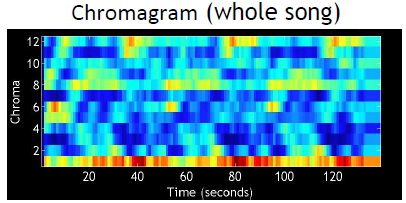
\includegraphics[width=3in]{Images/chroma}
				\end{center}
				%
				\alinea Le chromagramme tel quel a un problème : il \hl{dépend de la précision de la FFT utilisée}. En effet, les fréquences
					(discrètes) détectées par la FFT peuvent être un peu décalées par rapport aux fréquences des notes de musique.
					Le chromagramme peut être utilisé pour reconnaître les accords, la clé de la musique, les émotions données par la musique,
					ou encore pour analyser les musiques qui vont bien ensemble (utilisent la même suite d'accord).
				%
			%
			\subsubsection{Rythme}
				\alinea Contrairement aux deux précédentes dimensions, \hl{le rythme s'analyse sur plusieurs secondes de musique}, un 
					beat n'a de sens qu'avec les beats qui l'entourent pour finalement former un rythme. C'est pourquoi on va 
					\hl{analyser des mesures}.
				%
				\begin{center}
					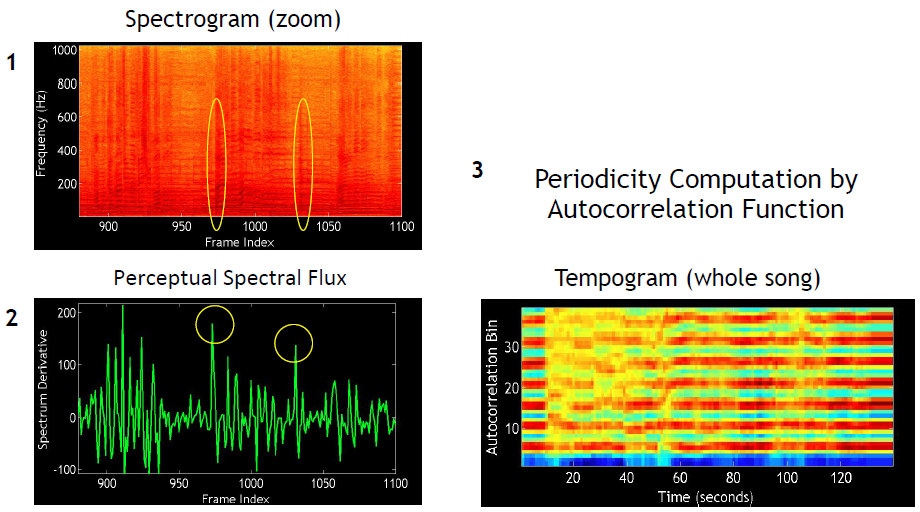
\includegraphics[width=5.2in]{Images/tempo} 
				\end{center}
				\begin{center}
					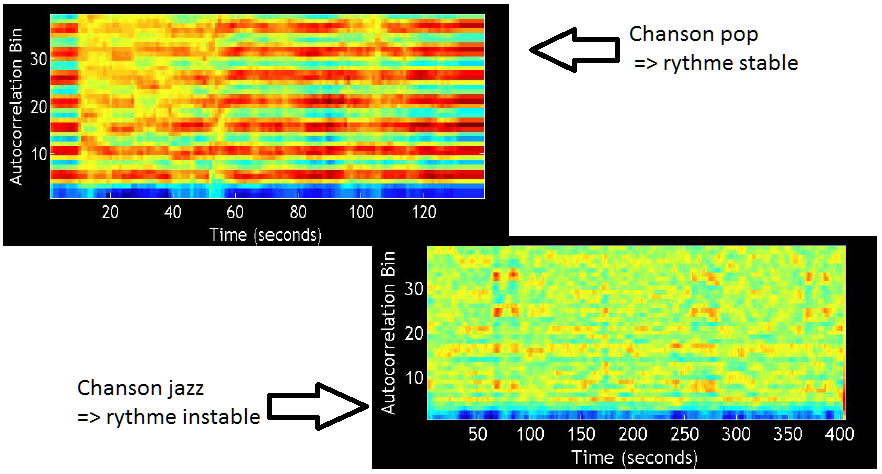
\includegraphics[width=4.66in]{Images/tempo2}
				\end{center}
				%			
				\alinea Le \hl{flux spectral perceptuel} représente un graphe de changement local. A chaque pic, on dit qu'il y a un 
					\hl{nouvel "event"}. C'est pourquoi les parties de chanson avec une batterie forte présentent des pics réguliers et 
					donc un tempogramme régulier. Il y a plusieurs lignes à cause des multiple de la période (genre 2$\pi$, 4$\pi$, ...). 
					Pour rectifier le tir, on va utiliser un \hl{tempogramme cyclique} dont les ordonnées $\in [1, 2]$ car on retient tout 
					ce qui se trouve entre le tempo de base (1) et ses multiples (2).
				%
				\begin{center}
					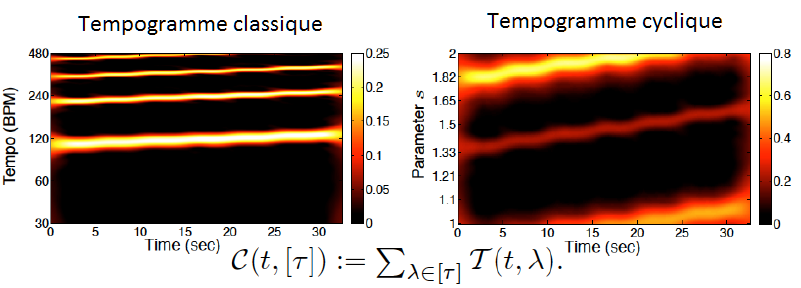
\includegraphics[width=5in]{Images/tempograms}
				\end{center}
				%
				\alinea On peut utiliser les tempogrammes pour \hl{segmenter les musiques} en différentes parties. On peut imaginer 
					qu'à chaque changement de rythme, une nouvelle partie de la musique commence
				%
				\begin{center}
					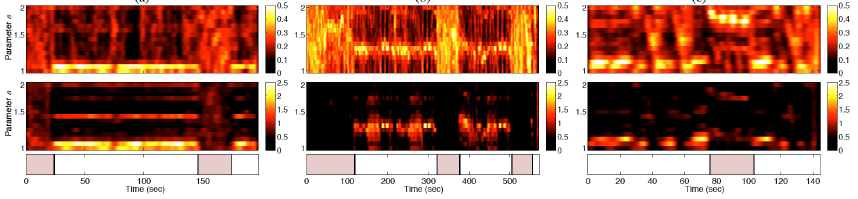
\includegraphics[width=\textwidth]{Images/segmentation}
				\end{center}
				%
			%
			\subsubsection{En bref}
				\alinea Grâce au timbre (timbregramme), aux notes (chromagramme) et au rythme (tempogramme), on peut essayer de classer
					des musiques selon leur genre et selon les émotions qu'elles évoquent.
				%
				\begin{center}
					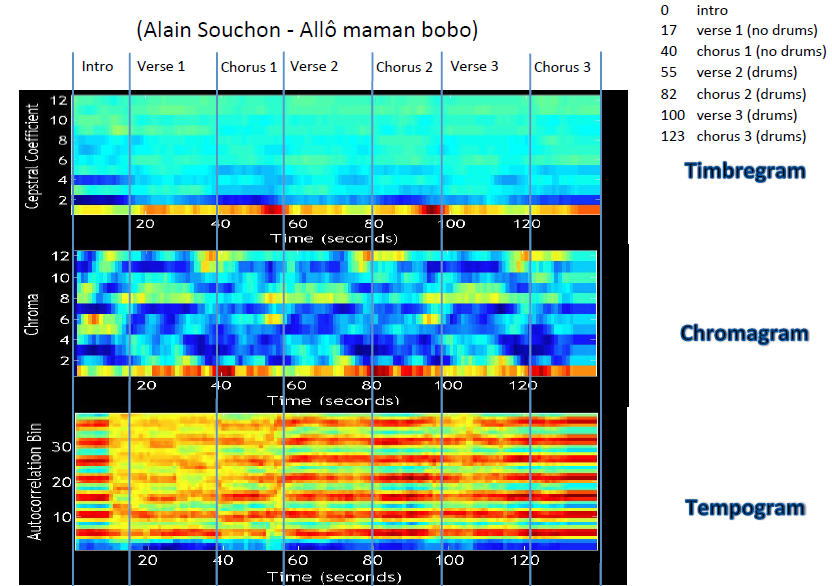
\includegraphics[width=5in]{Images/local_summary}
				\end{center}
				%
			%
		%	
		\subsection{Débuts de segment (onset)}	
			\alinea Cette partie est consacrée au calcul du flux spectral perceptuel. En effet, on a besoin de \hl{détecter le début de chaque
				note jouée} pour pouvoir estimer le début d'un nouvel "event". Cela pose \hl{quelques problèmes à résoudre} : 
				\begin{itemize}
					\setlength\itemsep{0cm}
					\item Séparer les notes de plusieurs instruments qui jouent en même temps.
					\item Combler le manque de démarcation claire (note qui change sans impulsion claire).
					\item Ne pas considérer un arrêt soudain d'une note comme un nouvel "event".
				\end{itemize}
			%
			\alinea La création de la fonction de détection d'onset (onset strength function) s'appelle aussi la \hl{réduction} car on 
				part d'un signal audio complet pour obtenir un signal réduit ne comprenant que des probabilités d'avoir un onset à un 
				moment donné (car on va avoir une valeur toutes les 10ms environs, donnant une fréquence de 100Hz).\\
			%
			\begin{minipage}{0.55\textwidth}
				\alinea Il y a trois chose que l'on peut faire pour la partie "réduction".
				\begin{itemize}
					\setlength\itemsep{0cm}
					\item Détecter les changements temporel (saut d'énergie soudain).
					\item Détecter les changements spectraux (changements nets dans des fft sur de courtes périodes).
					\item Utiliser des modèles probabilistes.
				\end{itemize}
			\end{minipage} \hfill
			\begin{minipage}{0.35\textwidth}
				\hl{\ \ \ \ \ \ \ \ \ \ \ \ \ \ \ \ \ \ \ \ \ \ \ \ \ \ \ \ \ \ \ \ \ \ \ \ \ \ \ \ \ \ \ \ \ \ \ \ \ \ \ \ \ \ \ \ \ \ }
				\begin{center}				
					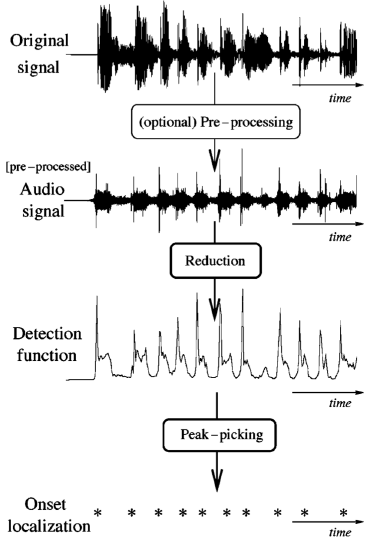
\includegraphics[width=\textwidth]{Images/onset}
				\end{center}
				\hl{\ \ \ \ \ \ \ \ \ \ \ \ \ \ \ \ \ \ \ \ \ \ \ \ \ \ \ \ \ \ \ \ \ \ \ \ \ \ \ \ \ \ \ \ \ \ \ \ \ \ \ \ \ \ \ \ \ \ }
			\end{minipage}~\\~\\~\\
			%
			\subsubsection{Variation d'énergie}
				\alinea On ne peut pas toujours détecter les onset par la dérivée de l'énergie car les notes sont parfois toutes
					connectées
				%
				\begin{center}
					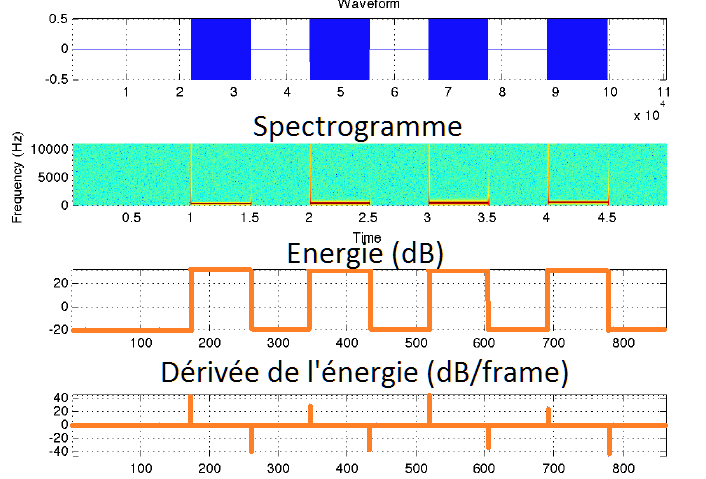
\includegraphics[width=0.49\textwidth]{Images/onset-ex} 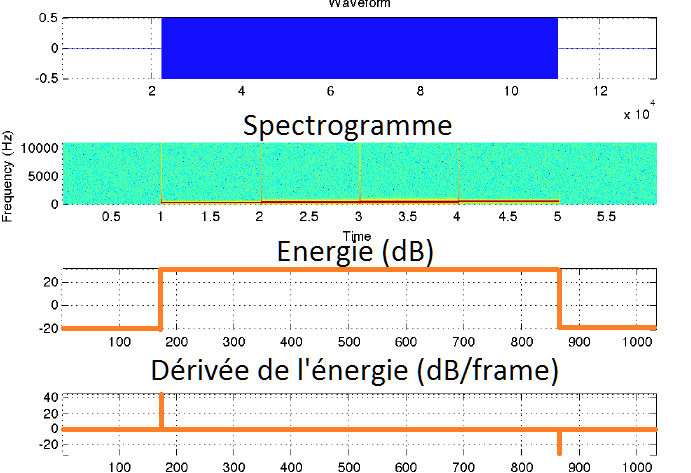
\includegraphics[width=0.49\textwidth]{Images/onset-ex2}
				\end{center}
				%
				\alinea Pour remédier à ce problème, on peut \hl{amplifier l'amplitude des hautes fréquences} dans le spectre afin de 
					marquer les changements abrupts. En effet, \hl{un changement soudain implique une montée d'énergie dans les hautes
					fréquences}. C'est ce qu'on a fait dans l'exemple suivant; on a calculé l'énergie sur le spectre amplifié en hautes
					fréquences. 
				%
				\begin{center}
					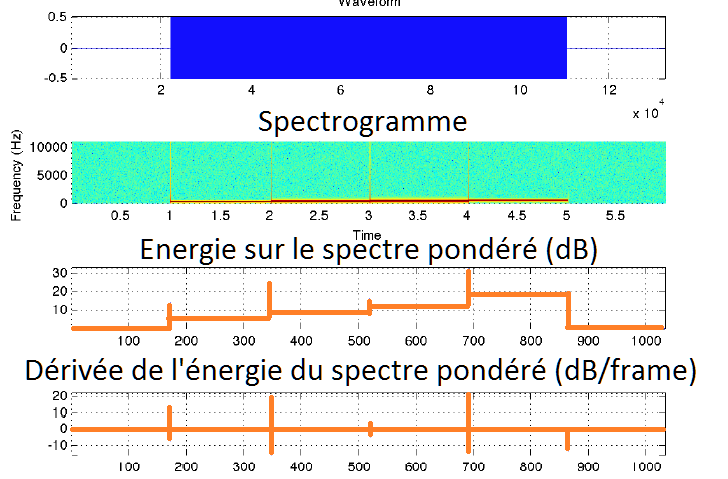
\includegraphics[width=0.49\textwidth]{Images/onset-amplified}
				\end{center}
				%
			%
			\subsubsection{Variations spectrales}
				\alinea On va ici regarder les changements entre des FFT consécutives. On va donc faire la \hl{différences entre plusieurs
					FFT}. On ne \hl{garde que les différences positives} (et on retourne 0 sinon) car on cherche de nouvelles fréquences 
					( si nouvelle - ancienne > 0 alors il est possible qu'une nouvelle note soit jouée). On finit par trouver des 
					changements de fréquence fondamentale en accumulant ces différences pour chaque bande de fréquence.
				%
				\begin{center}
					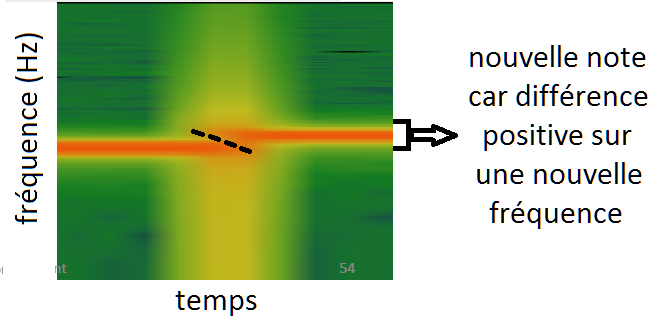
\includegraphics[width=3in]{Images/spectral}
				\end{center}
				%
				\alinea On a encore un problème à ce niveau-ci : Si un joueur de violon \hl{rejoue une même note}, on doit pouvoir détecter
					la nouvelle note, mais la différence spectrale n'y verra rien car ce seront presque les même composantes en fréquences 
					qui seront jouées. Par contre, on aura un \hl{changement de phase} car on recommence à jouer la note.\\
				%				
				~\\			
				%
				\alinea \hl{Une analyse trame par trame implique que la phase va changer à chaque analyse. Cependant, on peut prédire la phase
					de la prochaine analyse car elle augmente de manière linéaire jusqu'à retomber à zéro (évolution cyclique).}
					On va donc estimer qu'il y a une nouvelle note lorsqu'il y a \hl{un changement abrupt (non-linéaire, différent de la
					valeur prédite) de phase}. Tout ceci est illustré dans l'exemple suivant.
				%
				\begin{center}
					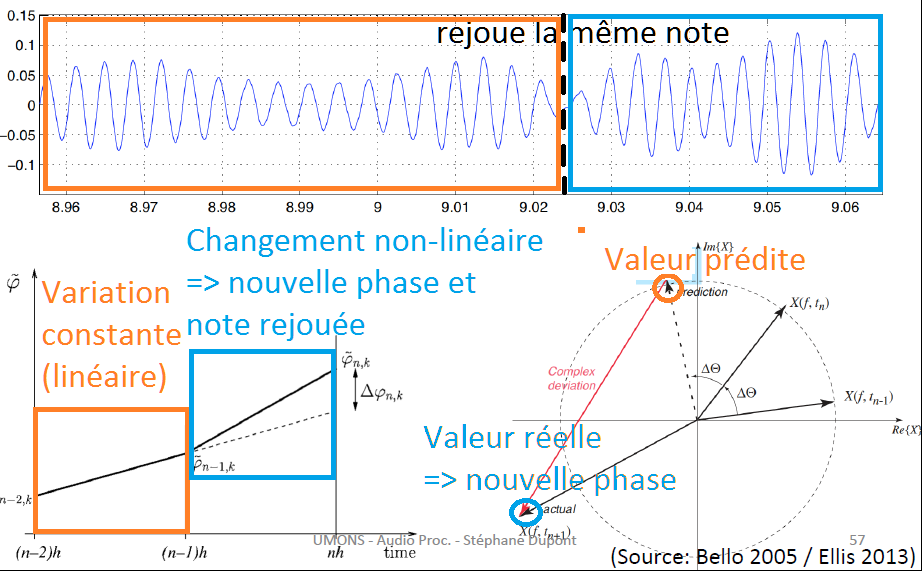
\includegraphics[width=\textwidth]{Images/phase}
				\end{center}
				%
				\alinea En pratique on a besoin de faire une analyse complexe de spectre dans la différence de fréquence et analyse de phase
					car sinon, la phase pourrait être trop sensible au bruit.
				%
			%
			\subsubsection{Sélection d'onset}
				\alinea Une fois que la fonction de détection d'onset est établie, il faut sélectionner les pics qui seront considérés comme
					onset, et donc comme début de segment. Ça peut se faire par une technique de \hl{sélection par seuil} ou par \hl{sélection
					intelligente de pic}. Cependant, un traitement supplémentaire est nécessaire avant de pouvoir faire cela. Un 
					\hl{post-traitement de la fonction de détection} est nécessaire afin de palier au changement d'orchestration de la chanson
					qui pourrait influencer la qualité des pics. On peut y appliquer un filtre passe-bas pour la lisser, un filtre passe haut 
					pour mettre en évidence les pics, on peut aussi la normaliser par l'écart-type, ...
				%
			%
			\subsubsection{\'Evaluation des performances}
				\alinea Deux méthodes sont utilisées en général pour évaluer les performances d'un détecteur : Précision/Rappel et la 
					F-mesure. La F-mesure valant $\frac{2 \cdot Precision \cdot Recall}{Precision + Recall}$
				%
				\begin{center}
					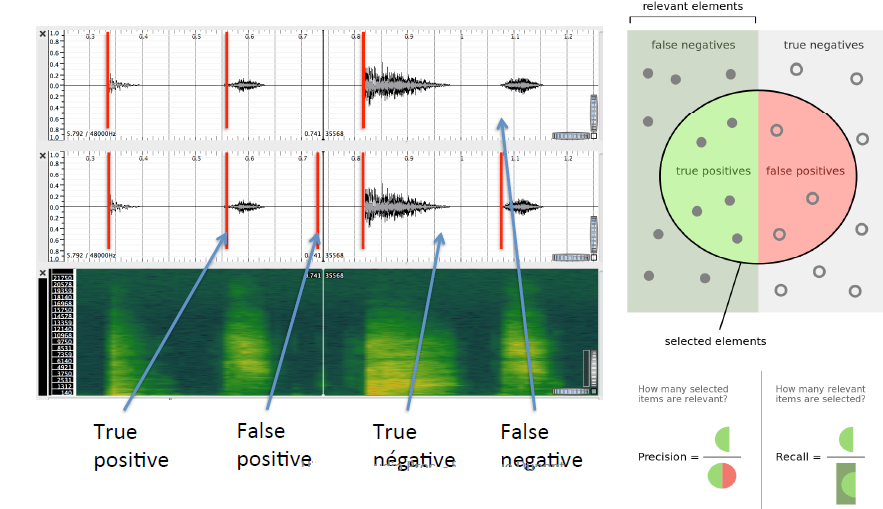
\includegraphics[width=\textwidth]{Images/precision}
				\end{center}
				%
			%
		%
		\subsection{Tempo}
			\alinea Jusqu'à présent, on s'est intéressé au rythme de manière locale, mais on voudrait maintenant avoir le \hl{tempo global} 
				de la chanson (e.g. 90BPM). Pour ce faire il faut détecter les onset. De plus, il faut s'intéresser aux "tatum", qui sont 
				des onsets entre les beats importants pour la perception. Typiquement, le \red{tempo} représente \hl{la périodicité entre 
				les onsets de grande intensité.}
			%
			\subsubsection{Méthode initiale}
				\alinea A la base, la recherche du tempo se faisait par \hl{recherche de fréquence}. On soumettait les onsets à des
					\hl{résonateurs}, qui cherchaient à quelle fréquence les résonateurs résonnaient le mieux. 				
				%
			\subsubsection{Approche d'auto-corrélation}
				\alinea On va chercher la\hl{ corrélation entre les onsets} en faisant glisser le graphe avec un certain délai à faire varier 
					(on superpose un onset avec tous les autres, mais décalés, pour connaître sa corrélation avec ceux là). 
					Le résultat donne les tempo possibles, mais avec les "octaves"
					possibles. C'est pourquoi on va pondérer le tout selon les tempo les plus utilisés en musique ou pour le genre musical en
					question (\hl{introduction de connaissance musicale}).
				%
				\begin{center}
					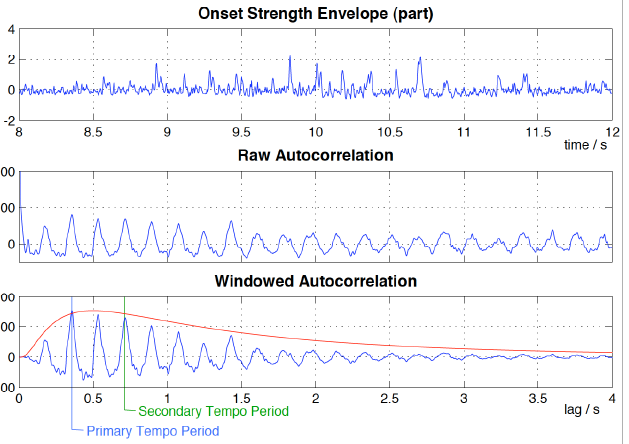
\includegraphics[width=5in]{Images/tempo3}
				\end{center}
				%
			%
		%
		\subsection{Beats}
			\alinea Une fois le tempo détecté, on peut s'attaquer à la détection des \red{beats} qui ne sont finalement que les 
				\hl{pics principaux d'onset séparés par des périodes de tempo}. Il faut donc chercher à \hl{maximiser la fonction}
				$$ \text{onsets} + \alpha \cdot \text{régularité du tempo} $$
				$\alpha$ étant un facteur d'échelle, permettant de l'importance de la régularité du tempo. Le problème est que 
				cette fonction demande un temps exponentiel à maximiser. On va donc avoir recours à de la \hl{programmation dynamique}
				(stocker les résultats intermédiaires parce qu'ils se répètent dans les formules) afin de résoudre le problème
				de manière itérative. Une autre technique utilisée est de faire la corrélation des onsets avec un modèle collant au 
				tempo, avec une certaine tolérance à l'erreur.\\
			%
			~\\
			%
			\alinea Une chose plus compliquée à faire est de détecter les \red{downbeats}, qui sont les \hl{beats qui démarrent une mesure}.
				Pour ce faire, o\hl{n a besoin de plus de connaissances musicales} car sa position varie selon les genres musicaux.
				Des fonctions de signatures temporelles seraient nécessaires.
			%
		%
		\subsection{Conclusion}		
			\alinea Note générale sur l'analyse musicale: 
				\hl{Il y a beaucoup plus de techniques que celles vues au cours pour extraire des informations d'une musique.}
			%
		%
	%
	\section{Identification de musique}
		\alinea Principe : reconnaître une musique par son titre et artiste en n'écoutant que quelques secondes.
			Pour ce faire on va chercher une "empreinte digitale" unique pour la musique, qui pourra être reconnue en écoutant
			une partie de la musique.
		%
		\begin{center}
			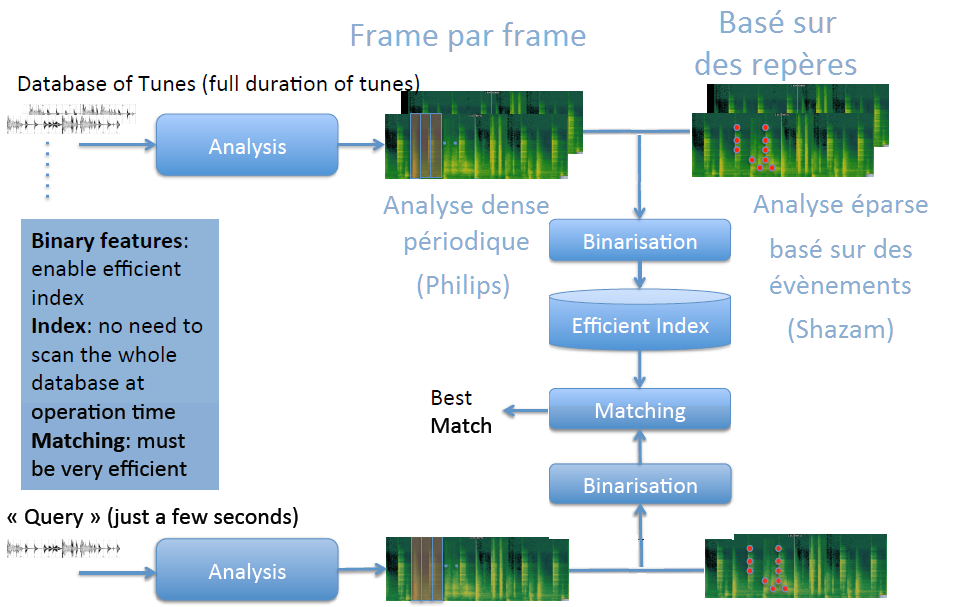
\includegraphics[width=6in]{Images/music_ID}
		\end{center}
		%
		\subsection{Analyse par frame}
			\alinea La méthode initiale consiste à \hl{encoder chaque frame sur 32 bits}. Les 32 bits représentent chacun une \hl{bande 
				de fréquence d'une FFT}. Pour chaque bande, s'il y a un \hl{changement local} conséquent par rapport à la FFT précédente, le 
				bit correspondant est mis à 1. Cette analyse se fait sur des frames plus longues que d'habitude ($\sim$100ms) afin 
				d'être plus \hl{robustes}.
			%
			\begin{center}
				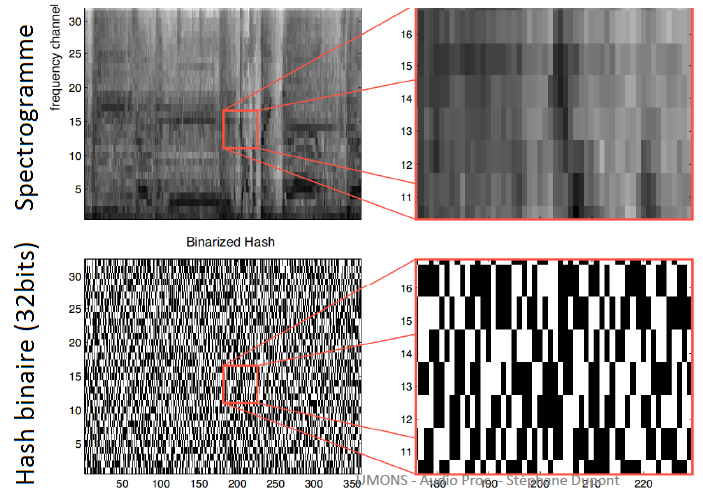
\includegraphics[width=3in]{Images/binary}
			\end{center}
			%
			\alinea On utilise ensuite ces 32 bits par frame pour retrouver la musique. La méthode principalement utilisée est une 
				"\hl{lookup table}" (LUT) qui a une table d'entrée contenant toutes les combinaisons possibles d'empreintes 32 bits
				($2^32$ possibilités). On a ensuite accès à n'importe quel endroit de n'importe quelle chanson et on peut 
				commencer à chercher un match.
			%
			\begin{center}
				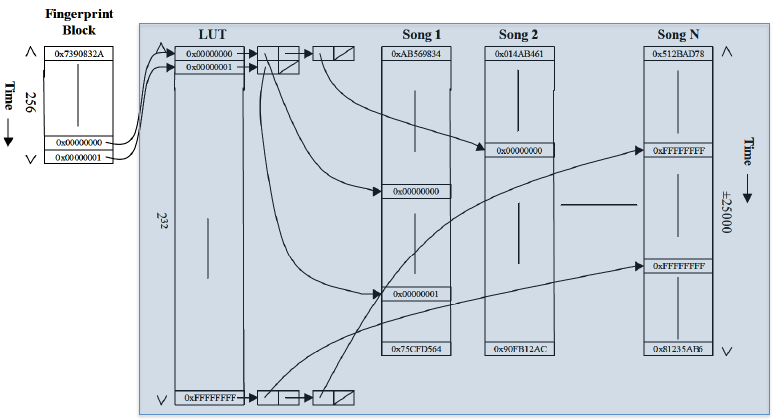
\includegraphics[width=\textwidth]{Images/LUT}
			\end{center}
			%
			\alinea En effet, utiliser une recherche en \hl{force brute est débile et prendrait trop de temps}. De plus, grâce à la LUT,
				on peut facilement contourner les \hl{erreurs à 1 bit près}. En inversant un par un les bits d'une séquence de 32 bits,
				on obtient 32 nouvelles séquences que l'on peut entrer dans la LUT. Néanmoins, \hl{le bruit peut poser problème} pour 
				retrouver correctement ces vecteurs 32 bits.
			%
		%
		\subsection{Analyse par repères (landmarks)}
			\alinea Le principe est de prendre un spectrogramme (fig. 1A), d'en \hl{extraire les pics}, et de se servir de chaque pic
				comme "\red{ancre}" (anchor) (fig. 1B). On va ensuite \hl{relier chaque ancre avec les autres pics (fig. 1C) et 
				former des triplets} \hl{(fréquence de démarrage, fréquence de fin, différence de temps)} (fig. 1D). Ce sont ces 
				triplets qui vont former nos repères dans la reconnaissance de musique. En pratique, on a pas besoin de trouver 
				beaucoup de landmarks communs pour identifier une musique.\\
			%
			~\\
			%
			\alinea Ces \hl{repères sont robustes} car ils se reposent sur les pics du spectrogramme qui sont les fréquences principales 
				et les harmoniques de celles-ci, et sont donc les \hl{composantes les plus fortes en énergie dans le spectre}. 
				Les valeurs des triplets sont discrétisées selon \hl{256 bandes de fréquences et 64 marquages temporels}.\\
				On a alors \hl{22 bits par repère} (fréquence, fréquence, temps) $\rightarrow$ (8 bits, 8 bits, 6 bits).
			%
			\begin{center}
				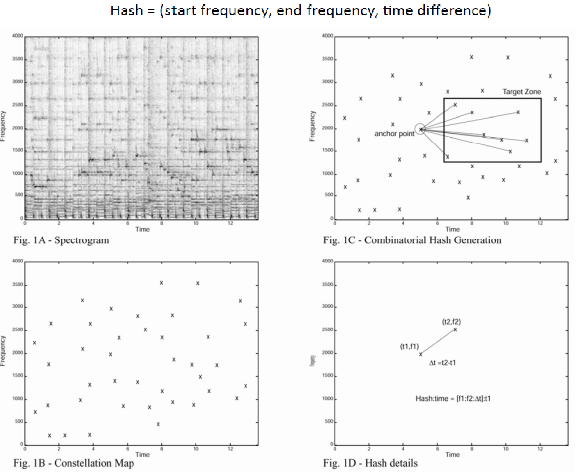
\includegraphics[width=\textwidth]{Images/landmark}
			\end{center}
			%
			\alinea La \hl{détection de pics dans le spectrogramme peut être ajustée} en réglant des paramètres afin de détecter moins ou plus 
				de pics, et ce afin de limiter le nombre de repères par chanson. Si de tels paramètres sont utilisés pour les chansons
				dans la base de données, alors ces paramètres doivent être appliqués également aux chansons écoutées (qui doivent être
				reconnues).\\
			%
			~\\
			%
			\alinea Ensuite, les repères sont présentés à une LUT qui va encore une fois retourner toutes les chansons qui contiennent
				le repère donné. Cependant,\hl{ pour reconnaître la musique, il va falloir faire appel au temps dans la chanson auquel 
				l'ancre du repère a été détecté}. En effet, on va faire une comparaison temporelle entre le moment où le (l'ancre du) 
				repère a été détecté et le moment ou le repère se trouve dans la chanson de la base de données.
				La comparaison devrait donner une séquence claire, permettant d'avoir un grand nombre de match sur une courte période,
				et donc un grand nombre de match dans un histogramme comptant le nombre de matchs par fenêtre de temps.
			%
			\begin{center}
				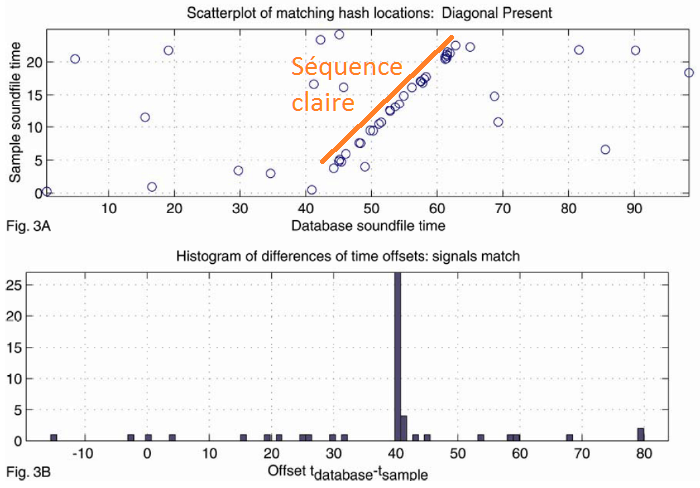
\includegraphics[width=5in]{Images/landmark2}
			\end{center}
			%
			\alinea Cette technique permet d'obtenir de \hl{très bon résultat, malgré un bruit élevé} (SNR de 3dB) et une compression
				élevée. Par contre, \hl{la technique est sensible à la modification de la vitesse} de la musique originale (car le repère 
				dépend du temps de par sa 3$^{\text{`eme}}$ composante) \hl{ou si on modifie le pitch de la musique} (car le repère dépend
				fortement des fréquences fondamentales).
			%
		%
	%
	\section{Réseaux de neurones (profonds)}
		\alinea Pour cette partie, c'est la reconnaissance vocale (ASR) qui va être étudiée. La technique de base pour faire de l'ASR
			consiste à suivre \hl{3 étapes} :
			\begin{enumerate}
				\setlength\itemsep{0cm}
				\item Extraire des informations utiles des fichiers audio (FFT, Spectrogramme, ...).
				\item Calculer les probabilités d'obtenir tel ou tel phonèmes à partir des informations extraites.
				\item Calculer les probabilités d'obtenir un tel mot ou une telle phrase selon une suite de phonèmes.
			\end{enumerate}
		%
		\alinea Les deux principales faiblesses de cette technique est (1) qu'il faut \hl{évaluer à la main l'utilité des informations} à
			extraire de l'audio \hl{pour chaque nouvelle tâche} et (2) qu'il n'y a \hl{pas d'optimisation globale} de ces 3 étapes, 
			il n'y a qu'une optimisation locale pour chaque étape. De plus, \hl{les performances n'égalent pas les performances humaines}.
			Pour remédier à ces problèmes, on va faire appel à des \hl{réseaux de neurones profonds qui vont effectuer les 3 étapes eux-même},
			permettant une optimisation globale et une facilité d'utilisation (car pas d'analyse des features intéressantes).
			Ce faisant, \hl{on se débarrasse de la partie analyse du signal}, mais aussi des \hl{suppositions} faites sur les 
			\hl{modèles probabilistes} et sur \hl{les features qui pourraient être intéressantes}.
		%
		\subsection{Neurone}
			\alinea Avant de créer un réseau, on va commencer par définir ce qu'est un neurone. Deux fonctions intéressaient les chercheurs 
				à la base : (1) \red{le symbolisme}, permettant de représenter les données et la connaissance humaine, et (2) 
				\red{le connectionisme}, permettant à des cellules virtuelles d'interagir et leur capacité d'apprentissage.\\
			%
			~\\
			%
			\alinea Le principe d'un \red{neurone} est de faire une \hl{somme pondérée de toutes les dimensions} de la donnée entrée,
				d'y ajouter éventuellement un \hl{\textit{bias},} et ensuite d'y \hl{appliquer une fonction} permettant
				de classer la donnée comme appartenant (1) ou n'appartenant pas (0) à une classe spécifique. On a donc un
				\hl{classificateur binaire}. On peut noter que si les données ne sont pas séparable linéairement, on peut
				toujours trouver une \hl{transformation de l'espace} (en ajoutant des dimensions par exemple) pour rendre les 
				données séparables linéairement dans ce nouvel espace.
			%
			\begin{center}
				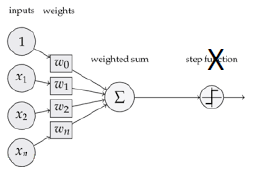
\includegraphics[width=3in]{Images/neuron}
			\end{center}
			%
			\alinea Entraîner un tel réseau consiste à \hl{ajuster les poids} de la somme. On peut noter que si un ensemble de poids
				classifie parfaitement un ensemble de donnée, ces même poids multipliés par une constante classifiera les données
				tout aussi parfaitement. Il n'y a donc \hl{pas de moyen de connaître les poids réellement optimaux} (car bases de donnée
				finies et incomplètes par rapport aux données réelles possibles). Les techniques modernes cherchent à éviter ce problème
				au maximum.
			%
		%
		\subsection{Réseau}
			\alinea Il existe plusieurs architectures connues : 
			%
			\begin{center}
				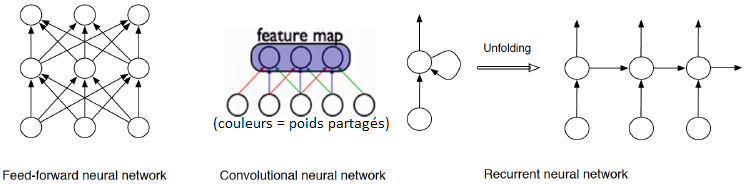
\includegraphics[width=\textwidth]{Images/networks}
			\end{center}
			%
			\alinea Lorsque beaucoup de neurones et de couches de neurones sot utilisées, il devient impossible d'ajuster les poids
				à la main. On va utiliser un algorithme de \hl{back-propagation} calculant des \hl{gradients} entre tous les poids
				et \textit{bias} afin de les ajuster de manière \hl{automatisée dans une phase d'apprentissage}. tout cela permettra
				 d'\hl{optimiser} une \hl{fonction de coût} utilisant ces paramètres.\\
			%
			~\\
			%
			\alinea \hl{On peut voir un neurone comme étant un filtre audio}, défini par ses poids, calculant se résonance avec  
				l'entrée (par un calcul de cross-corrélation). 
				Il en ressort une """"puissance de résonance"""", qu'on peut apparenter aux probabilité en sortie du neurone. 
				C'est par cette comparaison que l'on peut observer les résultats des couches intermédiaires d'un CNN.
				(On multiplie les pixels par les poids des neurones). On peut donc voir les \hl{réseaux de neurones comme une 
				manière de construire (durant la phase d'entraînement) d'appliquer une cascade, une banque de filtres.} 
			%
			\begin{center}
				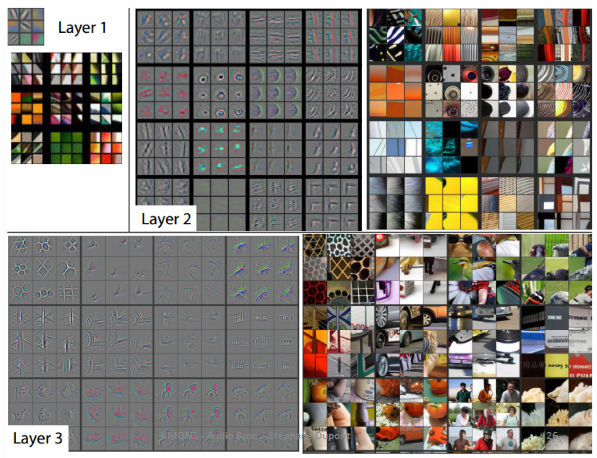
\includegraphics[width=4in]{Images/cnn}
			\end{center}
			%
			\subsubsection{Réseaux de neurones convolutionnels (CNN)}
				\alinea Les réseaux de neurones convolutionnels permettent de prendre des entrées avec énormément de dimensions.
					En effet, celui-ci :
					\begin{itemize}
						\setlength\itemsep{0cm}
						\item \hl{Regroupe les poids entre certains neurones} (pour simuler une convolution => appliquer un même filtre 
							à une zone de l'image). Ceci est plus ou moins équivalent à faire parcourir un seul neurone sur
							une zone de l'entrée (e.g. une zone d'image).
						\item Mets \hl{certains poids à 0 afin d'ignorer quelques dimensions} inutiles.
						\item A des \hl{couches de "pooling"} permettant de faire une moyenne des sorties de la couches précédentes
							et donc de réduire la taille du réseau progressivement \hl{($\sim$downsampling...)}. Pour ce faire,
							ces couches de pooling possèdent des neurones qui possèdent tous le même poids (parce que faire la moyenne
							c'est faire une somme pondéré avec un poids constant).
					\end{itemize}
				%
			%
		%
		\subsection{Reconnaissance audio}
			\alinea La technique de base utilisée est de calculer les \hl{MFCCs}. Cette technique est \hl{déjà inspirée par le biologique}
				(résolution des basses fréquences plus élevée par les filtres de Mel).
				
				
				L'image suivante illustre les étapes
				parcourue pour trouver ces coefficients : 
			%
			\begin{center}
				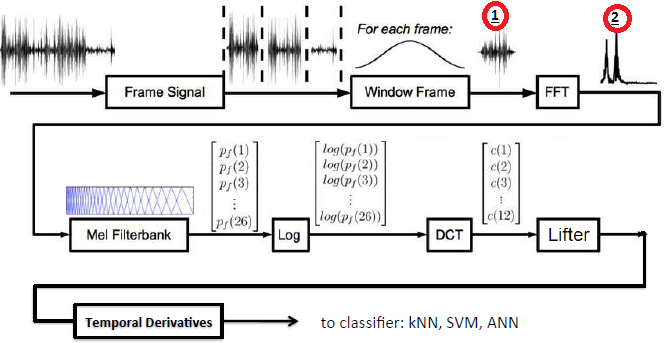
\includegraphics[width=6in]{Images/mfcc}
			\end{center}
			%
			\subsubsection{Amélioration 1}
				\alinea La première amélioration (cf. (1) dans l'image précédente) vise à mieux analyser le signal audio en utilisant 
					une Restricted Boltzmann Machine (\hl{RBM,
					une architecture de réseaux de neurones permettant un apprentissage non-supervisé}). Cette analyse va permette
					de creuser les détails de plusieurs bandes de fréquences en même temps. En effet, les \hl{phonèmes peuvent être
					détectés grâce à leurs deux fréquences de bases (formants)}, et les grouper déjà à ce niveau-ci permet une 
					analyse plus poussée.
				%
				\begin{center}
					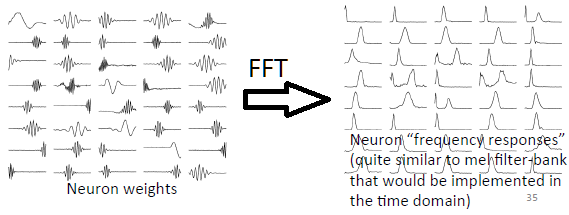
\includegraphics[width=5in]{Images/rbm}
				\end{center}
				%
			%
			\subsection{Amélioration 2}
				\alinea Une autre amélioration (cf. (2) de l'image sur les MFCCs) serait de ne pas analyser le signal audio 
					brut, mais d'\hl{analyser la sortie de la FFT} en la donnant en entrée à un réseau de neurones profond.
					Le but étant de \hl{remplacer la banque de filtre de Mel par des "filtres" calculés par un réseau de neurones}.
					On peut voir dans l'exemple suivant que les filtres obtenus sont très proches des filtres de Mel, et ces 
					derniers sont le résultats d'années de recherche dans le domaine. On a donc une structure qui permet de trouver
					les filtres \hl{optimaux} (ce qui n'était pas le cas pour les filtres de Mel) automatiquement, sans avoir 
					besoin d'années de recherche, juste de l'entraînement.
				%
				\begin{center}
					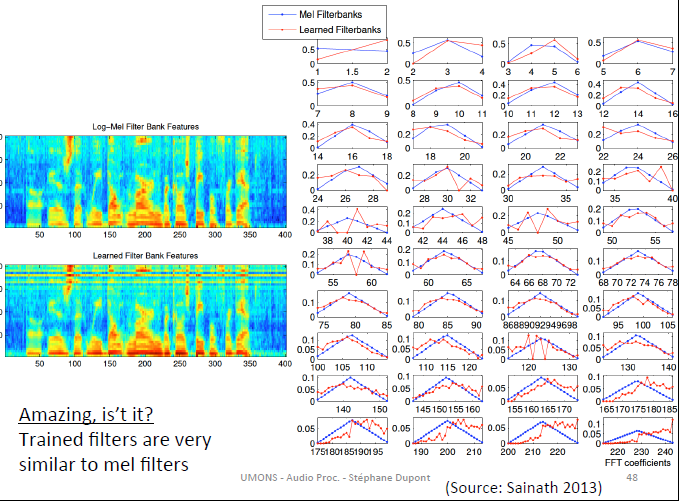
\includegraphics[width=5in]{Images/mel}
				\end{center}
				%
				\alinea Appliquer cette technique en sortie de la fenêtre de pondération (au (1) de l'image MFCC) également 
					permettrait d'améliorer encore les résultats.
				%
			%
			\subsubsection{Amélioration 3}
				\alinea Appliquer une RBM à la sortie de la FFT permet d'avoir des résultats assez haut-niveau en sortie. 
					(analyse fréquence par fréquence).
				%
			%
		%
		\subsection{Conclusion}
			\alinea Les réseaux de neurones profonds \hl{permettent d'entraîner automatiquement des systèmes complexes} "All-In-One", 
				mais \hl{demande énormément de données afin d'être précis}, peuvent vite \hl{devenir des boites noires}, et les étudier 
				demande \hl{beaucoup de temps car les architectures sont nombreuses} et encore en phase de tests.
			%
		%
	%
%
\pagebreak
%
\part{D'Alessandro -- Traitement audio matériel}
	\section{Question 1}
		\subsection{Question}
			\alinea \red{Décrivez les notions de “temps-réel” vues des points de vue du système informatique et de l’utilisateur. 
				À l’aide d’exemples concrets, illustrez brièvement comment ces deux perspectives affectent la latence acceptable d’un 
				système audio temps-réel.}
			%
		%
		\subsection{\'Eléments de réponse}
			\alinea %TODO Notes: hard real-time / human interaction + <1ms = confusion et >100?ms retard.
			%
		%
	%
	\section{Question 2}
		\subsection{Question}
			\alinea  \red{Vous êtes dans la situation où, pour produire un son en temps-réel, vous devriez allouer une ressource mémoire
				importante. On vous a dit, en passant, qu’il “fallait éviter les malloc(), car ça faisait glitcher l’audio”. 
				Veuillez re-contextualiser cette mise en garde: Qu’est-ce qu’un audio glitch? Quel est le lien entre allocation de 
				mémoire et audio glitch? Comment éviter cela?}
			%
		%
		\subsection{\'Eléments de réponse}
			\alinea %TODO priority inversion + ring buffer
			%
		%
	%
	\section{Question 3}
		\subsection{Question}
			\alinea \red{Comment, sur un système d’exploitation moderne, les applications gèrent-elles leur accès aux ressources audio? 
				Expliquer, dans son contexte, ce qu’est le “callback audio”, ce qu’il fait et son lien avec les entrées/sorties 
				audio d’un ordinateur typique.}
			%
		%
		\subsection{\'Eléments de réponse}
			\alinea %TODO shcéma buffer + interruptions.
			%
		%
	%
	\section{Question 4}
		\subsection{Question}
			\alinea \red{Dans mon application, j’ai inséré un filtre numérique très complexe et le calcul de ses coefficients prend, sur 
				une machine typique, 20 ms. Je souhaite bien évidement que le taux de rafraîchissement de ces coefficients soit le 
				plus proche possible du minimum, soit 50 Hz. Décrivez deux approches différentes permettant de réaliser ce filtrage 
				sans aucun glitch audio.}
			%
		%
		\subsection{\'Eléments de réponse}
			\alinea %TODO 1) Thread séparé + Ring buffer + atomic values 2) ?
			%
		%
	%
	\section{Question 5}
		\subsection{Question}
			\alinea \red{Décrivez en quoi la synthèse additive est un exemple simple de “phaseur + table d’onde” 
				( en anglais: “phasor + wavetable” ). À quoi le phaseur est-il associé en synthèse additive et pourquoi est-ce si 
				important de piloter la synthèse par ce phaseur?}
			%
		%
		\subsection{\'Eléments de réponse}
			\alinea %TODO revoir code CH1. /!\ humain sensible au changement de phase
			%
		%
	%
	\section{Question 6}
		\subsection{Question}
			\alinea \red{Qu’est-ce qu’un buffer circulaire ( ring buffer )? Illustrez son fonctionnement et son utilité dans deux exemples
				typiques: a) la visualisation de longs segments audio à l’écran; b) la synthèse de longues réponses impulsionnelles 
				hors du thread audio.}
			%
		%
		\subsection{\'Eléments de réponse}
			\alinea %TODO a) utilisation de la tête d'écriture dans la lecture audio => on peut lire longtemps sans dépasser la mémoire.
				    %TODO b) permet d'écrire la réponse impulsionnelle au fur et à mesure ?
			%
		%
	%
	\section{Question 7}
		\subsection{Question}
			\alinea \red{Décrivez le principe de fonctionnement d’un guide d’ondes ( en anglais: waveguide ) de type Karplus-Strong. 
				Pourquoi sonne-t-il comme une corde pincée? Quel mécanisme lui donne sa fréquence fondamentale? Comment est-elle calculée?}
			%
		%
		\subsection{\'Eléments de réponse}
			\alinea %TODO Revoir site internet du labo...
			%
		%
	%
%
\end{document}